\documentclass[tikz,border=5mm]{standalone}
\usepackage{pgfplots}
\usepackage{amsmath}
\pgfplotsset{compat=1.18}

% Explicit RGB color definitions
\definecolor{ogiveblue}{RGB}{0, 0, 255}
\definecolor{dotred}{RGB}{255, 0, 0}
\definecolor{projgreen}{RGB}{0, 100, 0}

\begin{document}
	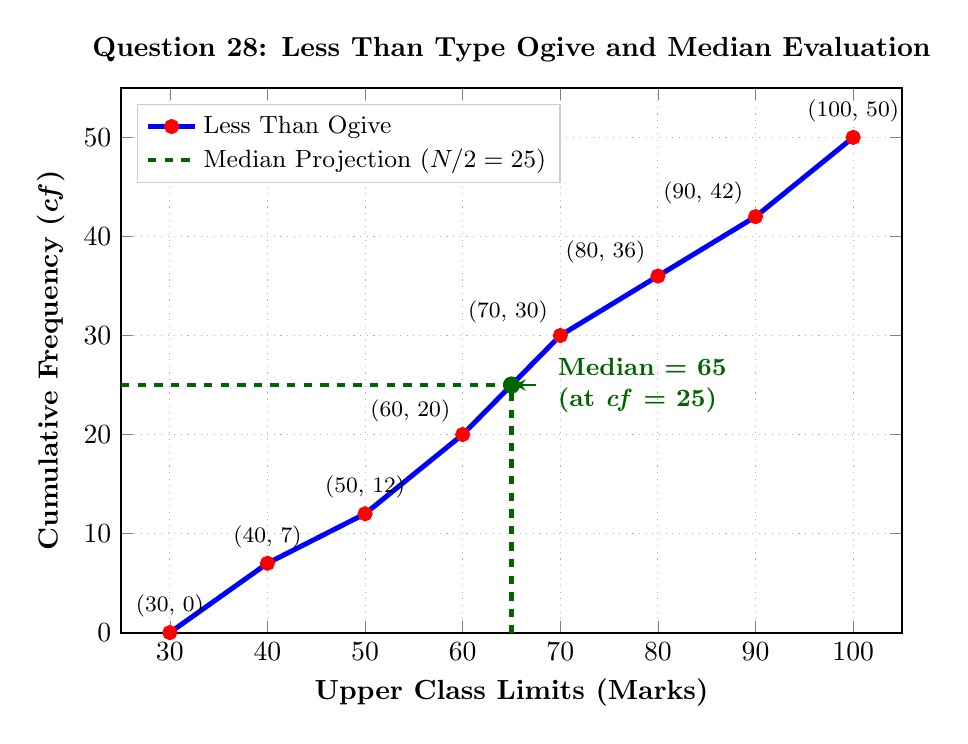
\begin{tikzpicture}
		\begin{axis}[
			width=11.5cm, height=8.5cm,
			title={\textbf{Question 28: Less Than Type Ogive and Median Evaluation}},
			xlabel={\textbf{Upper Class Limits (Marks)}},
			ylabel={\textbf{Cumulative Frequency (\textit{cf})}},
			xmin=25, xmax=105,
			ymin=0, ymax=55,
			xtick={30,40,50,60,70,80,90,100},
			ytick={0,10,20,30,40,50},
			grid=both,
			grid style={dotted, gray!60},
			axis line style={black, thick},
			legend cell align={left},
			legend style={at={(0.02,0.97)}, anchor=north west, font=\small, draw=gray!40}
			]
			% Ogive line with red dots
			\addplot[ogiveblue, line width=1.8pt, mark=*, mark options={fill=dotred, draw=dotred, scale=0.9}] coordinates {
				(30,0) (40,7) (50,12) (60,20) (70,30) (80,36) (90,42) (100,50)
			};
			\addlegendentry{Less Than Ogive}
			
			% Median projection dashed line
			\addplot[projgreen, dashed, line width=1.5pt] coordinates {
				(25,25) (65,25) (65,0)
			};
			\addlegendentry{Median Projection ($N/2 = 25$)}
			
			% Coordinate labels
			\node[above=2pt, font=\footnotesize] at (axis cs:30,0) {(30, 0)};
			\node[above=2pt, font=\footnotesize] at (axis cs:40,7) {(40, 7)};
			\node[above=2pt, font=\footnotesize] at (axis cs:50,12) {(50, 12)};
			\node[above left=1pt, font=\footnotesize] at (axis cs:60,20) {(60, 20)};
			\node[above left=1pt, font=\footnotesize] at (axis cs:70,30) {(70, 30)};
			\node[above left=1pt, font=\footnotesize] at (axis cs:80,36) {(80, 36)};
			\node[above left=1pt, font=\footnotesize] at (axis cs:90,42) {(90, 42)};
			\node[above=2pt, font=\footnotesize] at (axis cs:100,50) {(100, 50)};
			
			% Median green marker and annotation arrow
			\node[circle, fill=projgreen, inner sep=2.2pt] at (axis cs:65,25) {};
			\draw[<-, >=stealth, thick, projgreen] (axis cs:65.3, 25) -- (axis cs:67.5, 25);
			\node[anchor=west, font=\small, text=projgreen, inner sep=0pt] at (axis cs:68, 25) {
				\begin{tabular}{l}
					\textbf{Median = 65} \\
					\textbf{(at \textit{cf} = 25)}
				\end{tabular}
			};
		\end{axis}
	\end{tikzpicture}
\end{document}